\chapter{Documento de Especificação dos Casos de Teste} \label{documento_teste}

\begin{center}
 {\large Documento de Especificação dos Casos de Teste}\\[0.2cm]
 {BEViM}\\
 \end{center}

 \section*{Histórico de Alterações}
\begin{table}[h]
\centering
\begin{tabular}{|c|c|p{6cm}|p{5cm}|}
\hline
Data & Versão & Descrição & Responsável\\
\hline
01/11/2016 & 1.0 & Criação do documento. & Paulo Borba.\\
\hline
\end{tabular}
\end{table}

\section*{Introdução}

O documento de caso de teste serve para que o \textit{Product Owner} possa ter uma visão sobre as principais funcionalidades que seu sistema deverá ser testado. Serve como base para que a equipe de testadores possa se orientar e saber o passo a passo para criar um ambiente de teste e seguir o fluxo de passos para recriar a determinada situação da funcionalidade a qual será testada.

O sistema BEViM vai contar com alguns casos de testes que serão essenciais para garantir a integridade do sistema como um todo. Serão realizados testes das mais variadas formas e principalmente testes de integração para garantir a integração entre as frentes das engenharias desde o mais baixo nível até ao mais alto nível do sistema.

Todos os testes serão realizados em nível de software, a maioria deles só poderão ser realizados após a integração de todas as frentes de engenharias em um único produto. Esta é uma parte crítica pois é a comunicação entre as frentes que garantirão o sucesso das funcionalidades como um todo deste sistema.

O sistema BEViM é composto 3 componentes principais:
\newpage
\begin{itemize}
    \item Django-Web
    \begin{itemize}
        \item Trata-se da aplicação Web aonde o usuário irá se logar, poderá realizar vários ensaios de vibrações no produto que está em cima da bancada e por fim, poderá visualizar os dados coletados pelos sensores na forma de gráficos.
    \end{itemize}
    \item Django-Raspberry
    \begin{itemize}
        \item É a aplicação de servidor que irá se comunicar com a aplicação Web. Essa aplicação tem como objetivo organizar as requisições de ensaios para serem repassadas as rotinas de comunicação e, por fim, ler do banco de dados local para repassar os resultados a aplicação Web.
    \end{itemize}
    \item Rotinas de Comunicação e Parser
    \begin{itemize}
        \item São rotinas desenvolvidas para serem integradas com o Django da Raspberry com o objetivo de oferecer comunicação serial de modo simplificado. As rotinas de comunicação realizam a configuração da porta serial e permitem enviar e receber dados da malha de controle, e os dados recebidos são tratados pelo parser de forma a serem escritos no banco de dados.
    \end{itemize}
\end{itemize}

\subsection*{Modelo de dados}

Foi proposto um modelo de banco de dados tanto no sistema Web quanto na Raspberry, baseando-se no proposto de modelagem que o próprio Django oferece. Esta modelagem está de acordo com os dados que serão recebidos, tratados e exibidos para o usuário na forma de gráficos que serão consultados.

\begin{figure}[H]
\centering
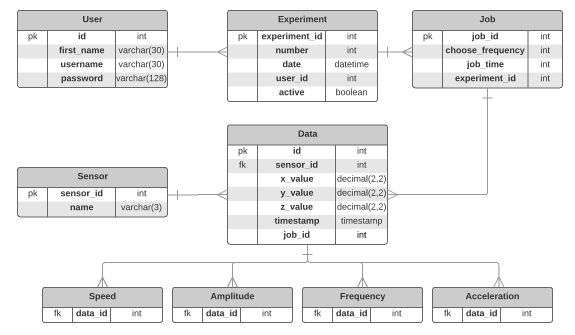
\includegraphics[keepaspectratio=true,scale=0.4]{figuras/visao_de_dados.png}
\caption{Modelagem dos dados da aplicação Web}
\label{fig:visao_de_dados_2}
\end{figure}

\begin{figure}[H]
\centering
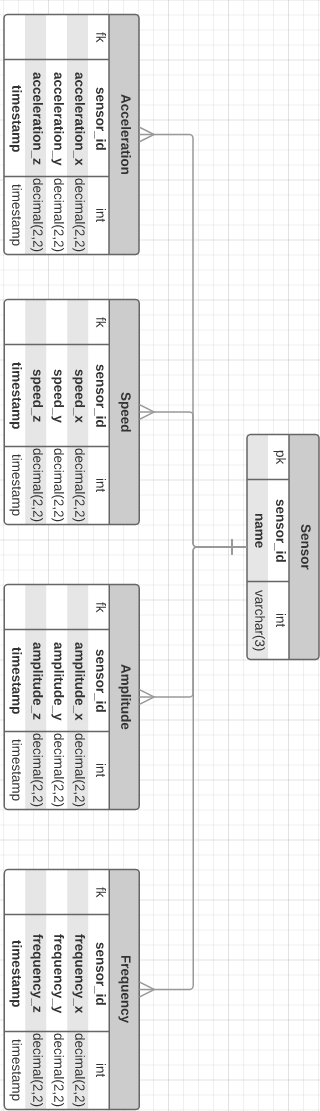
\includegraphics[keepaspectratio=true,scale=0.8]{figuras/banco-rasp.png}
\caption{Modelagem dos dados da aplicação Raspberry}
\label{fig:banco_rasp}
\end{figure}

\section*{Casos de Teste}

Este tópico tratará do detalhamento dos casos de testes e para fins de determinar a funcionalidade integra do sistema de acordo e alinhado aos requisitos definidos. Para isso explicaremos os tipos de testes que serão realizados na aplicação Web e na aplicação da Raspberry a fim de garantir essa integridade:

\begin{itemize}
    \item Teste de integração
        \begin{itemize}
            \item O teste de integração ele foca na funcionalidade parcial de um determinado subsistema integrado a outro (integração parcial) ou na funcionalidade total no sistema como um todo. Esse teste tem como objetivo saber se os requisitos estão de acordo com o que foi desenvolvido e esperado.
        \end{itemize}
    \item Teste caixa preta
        \begin{itemize}
            \item Esse teste é um teste ao qual o testador não tem noção do que se passa por dentro do sistema. O objetivo deste teste é testar saída do sistema para saber se estão de acordo com o esperado, sem se importa sobre como está sendo realizado as operações internas.
        \end{itemize}
\end{itemize}

Nas tabelas abaixo serão realizados descrição dos casos de teste de integração e caixa preta que irão determina a funcionalidade total do sistema, e quando os testes forem implementados e todos passarem será possível afirma que o sistema atende a todos os requisitos que foram levantados no inicio da elaboração deste projeto.

\begin{table}[H]
    \begin{center}
        \begin{tabular}{|p{5cm}|p{12cm}|}
            \hline
            \multicolumn{2}{|c|}{\textbf{Especificação de Caso de Teste}} \\ \hline
                \textbf{Projeto}                                        & BEViM - Web \\ \hline
                \textbf{Caso de Teste}                             & CT-01 \\ \hline
                \textbf{Tipo}                                             & Teste Caixa Preta \\ \hline
                \textbf{Propósito}                                     & Realizar o login do usuário \\ \hline
                \textbf{Descrição Geral}                           & Este teste valida como o sistema deverá se comporta caso o usuário e a senha sejam inválidos. O sistema foi projetado para realizar um tratamento de usuário e senha inválidos. \\ \hline
                \textbf{Insumos para o caso de Teste}    & O servidor Django tem que estar ativado. \\ \hline
                \textbf{Roteiro para realização do Teste}&  1. Realizar as migrações dos dados da model para o Banco de Dados local, 2. Criar um usuário de teste via terminal do banco de dados, 3. Levantar o servidor Django localmente, 4. Logar na página da aplicação com o usuário criado. \\ \hline
            \multicolumn{2}{|c|}{\textbf{Cenários de Teste}} \\ \hline
                \textbf{Objetivo Específico}                      & \textbf{Saídas Esperadas} \\ \hline
                Tratar o envio de usuário que não existe na base de dados. & Sistema deverá exibir uma exceção dizendo que o usuário não existe. \\ \hline
                Tratar a password errada. & Sistema deverá informa que a senha está errada e pedir para digite novamente. \\ \hline
        \end{tabular}
    \end{center}
    \caption[Caso de Teste - CT01]{Caso de Teste - CT01
    \protect Fonte: Autor}
    \label{CT-01}
\end{table}

\begin{table}[H]
    \begin{center}
        \begin{tabular}{|p{5cm}|p{12cm}|}
            \hline
            \multicolumn{2}{|c|}{\textbf{Especificação de Caso de Teste}} \\ \hline
                \textbf{Projeto}                                        & BEViM-Web \\ \hline
                \textbf{Caso de Teste}                             & CT-02 \\ \hline
                \textbf{Tipo}                                             & Teste de Integração \\ \hline
                \textbf{Propósito}                                     & Processamento do GET e POST do RESTful na aplicação \\ \hline
                \textbf{Descrição Geral}                           & Este teste valida como o sistema deverá se comportar no caso de receber uma requisição GET ou POST que não estejam disponíveis. O sistema foi projetado de forma que todas as requisições GET e POST estejam validas dentro do sistema local. \\ \hline
                \textbf{Insumos para o caso de Teste}    & O servidor Django tem que estar ativado. \\ \hline
                \textbf{Roteiro para realização do Teste}&  1. Subir o servidor Django, 2. Realizar uma requisição GET com um resultado cujo seja esperado e comparar se o resultado obtido é o mesmo do esperado, 3. Realizar uma requisição POST em uma página de forma a saber se o POST está funcionando devidamente. \\ \hline
            \multicolumn{2}{|c|}{\textbf{Cenários de Teste}} \\ \hline
                \textbf{Objetivo Específico}                      & \textbf{Saídas Esperadas} \\ \hline
                Tratar um GET cujo o resultado não é esperado & Sistema deverá realizar um tratamento do erro 404 e mostrar que tal recurso não está disponível \\ \hline
                Tratar o POST cujo o acesso não está sendo permitido & Sistema deverá tratar a permissão dizendo que não possui a permissão devida ou está indisponível.Sistema deverá tratar a permissão dizendo que não possui a permissão devida ou está indisponível. \\ \hline
        \end{tabular}
    \end{center}
    \caption[Caso de Teste - CT02]{Caso de Teste - CT02
    \protect Fonte: Autor}
    \label{CT-02}
\end{table}

\begin{table}[H]
    \begin{center}
        \begin{tabular}{|p{5cm}|p{12cm}|}
            \hline
            \multicolumn{2}{|c|}{\textbf{Especificação de Caso de Teste}} \\ \hline
                \textbf{Projeto}                                        & BEViM-Web e BEViM-Rasp \\ \hline
                \textbf{Caso de Teste}                             & CT-03 \\ \hline
                \textbf{Tipo}                                             & Teste de Integração \\ \hline
                \textbf{Propósito}                                     & GET e POST da aplicação Web, processadas na aplicação da Raspberry \\ \hline
                \textbf{Descrição Geral}                           & Este teste valida como o sistema deverá se comportar ao receber requisições de GET ou POST entre aplicações. O sistema foi projetado de forma que todas as requisições GET e POST sejam processadas de acordo com o que foi determinado. \\ \hline
                \textbf{Insumos para o caso de Teste}    & O servidor Django Web e da Raspberry tem que ambos estarem ativados. \\ \hline
                \textbf{Roteiro para realização do Teste}&  1. Subir o servidor Django web e da raspberry, 2. Realizar uma requisição POST via Web para Rasp de modo a testar a comunicação entre as aplicações, 3. Realizar uma requisição GET via Web para Rasp de mod a testar a comunicação entre as aplicações, 4. Agora realizar no sentido Rasp -> Web os passos 2 e 3 que foram realizados, 5. Realizar verificação da integridade dos dados comunicados, para saber se estão corretos \\ \hline
            \multicolumn{2}{|c|}{\textbf{Cenários de Teste}} \\ \hline
                \textbf{Objetivo Específico}                      & \textbf{Saídas Esperadas} \\ \hline
                Tratar no caso de perca de dados durante a comunicação & Sistema deverá pedir pela mesma informação novamente para garantir sua integridade \\ \hline
                Tratar no caso da falta de conexão entre ambos os sistemas & Sistema deverá informa ao usuário que não possui conexão com a internet, ou que o sistema ao qual está tentando se comunicar, está fora do ar. \\ \hline
        \end{tabular}
    \end{center}
    \caption[Caso de Teste - CT03]{Caso de Teste - CT03
    \protect Fonte: Autor}
    \label{CT-03}
\end{table}


\begin{table}[H]
    \begin{center}
        \begin{tabular}{|p{5cm}|p{12cm}|}
            \hline
            \multicolumn{2}{|c|}{\textbf{Especificação de Caso de Teste}} \\ \hline
                \textbf{Projeto}                                        & Rotinas de Comunicação e Parser e BEViM-Rasp\\ \hline
                \textbf{Caso de Teste}                             & CT-04 \\ \hline
                \textbf{Tipo}                                             & Teste de Integração \\ \hline
                \textbf{Propósito}                                     & Testar conexão, envio e leitura de dados com o Banco de Dados Django \\ \hline
                \textbf{Descrição Geral}                           & Este teste tem como objetvido validar a conexão com o banco de dados da Raspberry, bem como escrita e leitura desses dados. O sistema deve estar preparado para tratar caso a conexão com o banco falhe ou tenha um estouro de memória devido a quantidade de informações que estejam transitando esteja muito alta. \\ \hline
                \textbf{Insumos para o caso de Teste}    & O servidor Django Raspberry tem que estar ativo. \\ \hline
                \textbf{Roteiro para realização do Teste}&  1. Subir o servidor Django da raspberry, 2.Utilizando o Parser, realizar a conexão com o banco de dados local, 3. Realizar a inserção de um dado em uma tabela, 4. Realizar a leitura deste mesmo dado na tabela, 5. Averiguar se o dado guardado é o mesmo lido  \\ \hline
            \multicolumn{2}{|c|}{\textbf{Cenários de Teste}} \\ \hline
                \textbf{Objetivo Específico}                      & \textbf{Saídas Esperadas} \\ \hline
                Tratar caso a conexão com o banco de dados não seja estabelecida & Sistema deverá informa que o banco de dados local está corrompido devido algum problema de hardware/software que venha a ter prejudicado a integridade dos dados \\ \hline
                Tratar caso aconteça estouro de memória para evitar que o sistema trave devido a quantidade de informações transitando & Sistema deverá informa o percentual de uso da memória interna, do disco rígido e de processamento, e quando as 3 variáveis chegarem a um limite o sistema deverá lançar um anuncio ao usuário informando o risco de possível travamento do sistema. \\ \hline
        \end{tabular}
    \end{center}
    \caption[Caso de Teste - CT04]{Caso de Teste - CT04
    \protect Fonte: Autor}
    \label{CT-04}
\end{table}

\begin{table}[H]
    \begin{center}
        \begin{tabular}{|p{5cm}|p{12cm}|}
            \hline
            \multicolumn{2}{|c|}{\textbf{Especificação de Caso de Teste}} \\ \hline
                \textbf{Projeto}                                        & Rotinas de Comunicação e Parser e BEViM-Rasp\\ \hline
                \textbf{Caso de Teste}                             & CT-05 \\ \hline
                \textbf{Tipo}                                             & Teste de Integração \\ \hline
                \textbf{Propósito}                                     & Testar conexão, envio e leitura de dados com o Banco de Dados Django \\ \hline
                \textbf{Descrição Geral}                           & Este teste tem como objetvido validar a conexão com o banco de dados da Raspberry, bem como escrita e leitura desses dados. O sistema deve estar preparado para tratar caso a conexão com o banco falhe ou tenha um estouro de memória devido a quantidade de informações que estejam transitando esteja muito alta. \\ \hline
                \textbf{Insumos para o caso de Teste}    & O servidor Django Raspberry tem que estar ativo. \\ \hline
                \textbf{Roteiro para realização do Teste}&  1. Subir o servidor Django da raspberry, 2.Utilizando o Parser, realizar a conexão com o banco de dados local, 3. Realizar a inserção de um dado em uma tabela, 4. Realizar a leitura deste mesmo dado na tabela, 5. Averiguar se o dado guardado é o mesmo lido  \\ \hline
            \multicolumn{2}{|c|}{\textbf{Cenários de Teste}} \\ \hline
                \textbf{Objetivo Específico}                      & \textbf{Saídas Esperadas} \\ \hline
                Tratar caso a conexão com o banco de dados não seja estabelecida & Sistema deverá informa que o banco de dados local está corrompido devido algum problema de hardware/software que venha a ter prejudicado a integridade dos dados \\ \hline
                Tratar caso aconteça estouro de memória para evitar que o sistema trave devido a quantidade de informações transitando & Sistema deverá informa o percentual de uso da memória interna, do disco rígido e de processamento, e quando as 3 variáveis chegarem a um limite o sistema deverá lançar um anuncio ao usuário informando o risco de possível travamento do sistema. \\ \hline
        \end{tabular}
    \end{center}
    \caption[Caso de Teste - CT05]{Caso de Teste - CT05
    \protect Fonte: Autor}
    \label{CT-05}
\end{table}

\begin{table}[H]
    \begin{center}
        \begin{tabular}{|p{5cm}|p{12cm}|}
            \hline
            \multicolumn{2}{|c|}{\textbf{Especificação de Caso de Teste}} \\ \hline
                \textbf{Projeto}                                        & Rotinas de Comunicação e Parser e Arduino\\ \hline
                \textbf{Caso de Teste}                             & CT-06 \\ \hline
                \textbf{Tipo}                                             & Teste de Integração \\ \hline
                \textbf{Propósito}                                     & Testar conexão, escrita e leitura dos dados da simulação do sistema, comunicação entre Arduino e Raspberry \\ \hline
                \textbf{Descrição Geral}                           & Este teste tem como objetivo realizar teste de conexão via porta serial entre Raspberry e Arduino, utilizando a rotina de comunicação desenvolvida em Python. O sistema deve realizar a leitura e escrita dos dados de forma integra. \\ \hline
                \textbf{Insumos para o caso de Teste}    & Subir uma instância de leitura e uma instância de escrita em terminais diferentes, escrever o input da simulação e iniciar um experimento. \\ \hline
                \textbf{Roteiro para realização do Teste}&  1. Subir uma instância de pyserial em modo de leitura, 2. Subir uma instância de pyserial em modo de escrita, 3. Iniciar o experimento com -1 e logo em seguida com a frequência 10, 4. Observa o output do modo de leitura para saber se está de acordo com o que se espera da simulação. \\ \hline
            \multicolumn{2}{|c|}{\textbf{Cenários de Teste}} \\ \hline
                \textbf{Objetivo Específico}                      & \textbf{Saídas Esperadas} \\ \hline
                Tratar a perca de dados caso o sistema tenha package loss durante a comunicação & O sistema deverá pedir para o sistema enviar o pacote perdido novamente para leitura e assegurar que o dado chegado é o que se esperava da simuĺação \\ \hline
                Tratar da integridade dos dados obtidos  & O sistema deverá garantir uma integridade contínua dos dados de modo que estes dados tenham confiabilidade. \\ \hline
        \end{tabular}
    \end{center}
    \caption[Caso de Teste - CT06]{Caso de Teste - CT06
    \protect Fonte: Autor}
    \label{CT-06}
\end{table}

\begin{table}[H]
    \begin{center}
        \begin{tabular}{|p{5cm}|p{12cm}|}
            \hline
            \multicolumn{2}{|c|}{\textbf{Especificação de Caso de Teste}} \\ \hline
                \textbf{Projeto}                                        & BEViM-Rasp, BEViM-Web e Rotinas de Comunicação e Parser\\ \hline
                \textbf{Caso de Teste}                             & CT-07 \\ \hline
                \textbf{Tipo}                                             & Teste de Integração \\ \hline
                \textbf{Propósito}                                     & Realizar o teste da rotina de requerimento dos sensores ativos no sistema para repasse na aplicação Web \\ \hline
                \textbf{Descrição Geral}                           & Este teste possui uma integridade de alto nível, requerendo um maior cuidado. O objetivo é que a aplicação Web, faça uma requisição dos sensores ativos no sistema, essa requisição será repassada por internet ao BEViM-Rasp até as Rotinas de comunicação que irão iniciar escrita do comando para envio e a leitura dos sensores ativos, que serão lidos pelos métodos do Parser para escrita no banco de dados e por fim buscados por um GET da aplicação Web no banco de dados da Raspberry e atualizados no sistema que o usuário acessa. \\ \hline
                \textbf{Insumos para o caso de Teste}    & Subir os Djangos da Raspberry e da aplicação Web, e preparar a estrutura de comunicação com o Arduino ativo e conectado a Raspberry \\ \hline
                \textbf{Roteiro para realização do Teste}&  1. Subir djangos Web e Raspberry, 2. Ligar Arduino a Raspberry, 3. Repassar a requisição dos sensores ativos via aplicação Web, 4. Verificar se os sensores ativos batem com o que a simulação realmente enviou \\ \hline
            \multicolumn{2}{|c|}{\textbf{Cenários de Teste}} \\ \hline
                \textbf{Objetivo Específico}                      & \textbf{Saídas Esperadas} \\ \hline
                Garantir a funcionaldiade na totalidade das rotinas e do sistema integrado & O sistema deverá responder de acordo com a rotina iniciada, e caso algum problema ocorra durante sua execução a mesma deverá informa ao usuário a causa deste erro. \\ \hline
        \end{tabular}
    \end{center}
    \caption[Caso de Teste - CT07]{Caso de Teste - CT07
    \protect Fonte: Autor}
    \label{CT-07}
\end{table}

\begin{table}[H]
    \begin{center}
        \begin{tabular}{|p{5cm}|p{12cm}|}
            \hline
            \multicolumn{2}{|c|}{\textbf{Especificação de Caso de Teste}} \\ \hline
                \textbf{Projeto}                                        & BEViM-Rasp, BEViM-Web, Rotinas de Comunicação e Parser e Arduino \\ \hline
                \textbf{Caso de Teste}                             & CT-08 \\ \hline
                \textbf{Tipo}                                             & Teste de Integração \\ \hline
                \textbf{Propósito}                                     & Realizar o teste de 10 segundos de um job a uma frequência de 70hz e visualizar seu resultados nos gráficos \\ \hline
                \textbf{Descrição Geral}                           & Este teste têm como objetivo testar a principal função de envio de um comando, aguardo da leitura dos dados no tempo estabelecido e visualização dos dados na interface gráfica. O sistema têm que estar pronto para o grande volume de dados que será enviado a Raspberry, esses dados deverão ser tratados, e guardados na base de dados local, e por fim deverão ser lidos pelo GET da aplicação Web e repassados a interface sobre quais sensores estão ativos. \\ \hline
                \textbf{Insumos para o caso de Teste}    & Subir os Djangos da Raspberry e da aplicação Web, e preparar a estrutura de comunicação com o Arduino ativo e conectado a Raspberry \\ \hline
                \textbf{Roteiro para realização do Teste}&  1. Subir djangos Web e Raspberry, 2. Ligar Arduino a Raspberry, 3. Criar 1 job com duração de 10 segundos a um a frequencia de 70hz, 4. Averiguar os dados recebidos e os gráficos que foram montados  \\ \hline
            \multicolumn{2}{|c|}{\textbf{Cenários de Teste}} \\ \hline
                \textbf{Objetivo Específico}                      & \textbf{Saídas Esperadas} \\ \hline
                Tratar a exibição dos dados resultantes do experimento & O sistema web deverá preencher a base de dados com os dados resultantes e a aplicação deverá exibir o gráfico desses dados, bem como realizar o processamento desses dados e exibi-los logo em seguida. \\ \hline
        \end{tabular}
    \end{center}
    \caption[Caso de Teste - CT08]{Caso de Teste - CT08
    \protect Fonte: Autor}
    \label{CT-08}
\end{table}

\begin{table}[H]
    \begin{center}
        \begin{tabular}{|p{5cm}|p{12cm}|}
            \hline
            \multicolumn{2}{|c|}{\textbf{Especificação de Caso de Teste}} \\ \hline
                \textbf{Projeto}                                        & BEViM-Rasp, BEViM-Web, Rotinas de Comunicação e Parser e Arduino\\ \hline
                \textbf{Caso de Teste}                             & CT-09 \\ \hline
                \textbf{Tipo}                                             & Teste de Integração \\ \hline
                \textbf{Propósito}                                     & Realizar teste de 5 jobs com diferentes frequências e diferentes tempos e observar os resultados nos gráficos \\ \hline
                \textbf{Descrição Geral}                           & Este teste têm como objetivo realizar testes de multiplos jobs e frequências para saber se a Raspberry vai aguentar a quantidade de dados, memória e processamento das operações de input  e output em conjunto com a aplicação Web e o sistema de controle simulado pelo Arduino. \\ \hline
                \textbf{Insumos para o caso de Teste}    & Subir os Djangos da Raspberry e da aplicação Web, e preparar a estrutura de comunicação com o Arduino ativo e conectado a Raspberry \\ \hline
                \textbf{Roteiro para realização do Teste}&  1. Subir djangos Web e Raspberry, 2. Ligar Arduino a Raspberry, 3. Criar 5 jobs com durações aleatórias e de diferentes frequências, 4. Averiguar os dados recebidos e os gráficos que foram montados  \\ \hline
            \multicolumn{2}{|c|}{\textbf{Cenários de Teste}} \\ \hline
                \textbf{Objetivo Específico}                      & \textbf{Saídas Esperadas} \\ \hline
                Tratar a exibição dos dados resultantes do experimento & O sistema web deverá preencher a base de dados com os dados resultantes e a aplicação deverá exibir o gráfico desses dados, bem como realizar o processamento desses dados e exibi-los logo em seguida. \\ \hline
        \end{tabular}
    \end{center}
    \caption[Caso de Teste - CT09]{Caso de Teste - CT09
    \protect Fonte: Autor}
    \label{CT-09}
\end{table}

\begin{table}[H]
    \begin{center}
        \begin{tabular}{|p{5cm}|p{12cm}|}
            \hline
            \multicolumn{2}{|c|}{\textbf{Especificação de Caso de Teste}} \\ \hline
                \textbf{Projeto}                                        & BEViM-Rasp, BEViM-Web e Rotinas de Comunicação e Parser\\ \hline
                \textbf{Caso de Teste}                             & CT-10 \\ \hline
                \textbf{Tipo}                                             & Teste de Integração de todo o Sistema Integrado \\ \hline
                \textbf{Propósito}                                     & Realizar teste de 10 jobs com diferentes frequências e diferentes tempos e observar os resultados nos gráficos e que estejam integrados com todas as frentes de engenharia em um único produto \\ \hline
                \textbf{Descrição Geral}                           & Este teste têm como objetivo testar o sistema como um todo desde o seu envio de requisição do job juntamente com a frequência e o inicio do experimento na bancada, e a alternância de jobs, a comunicação entre as diferentes frentes desde a estrutura, eletro-mecânica, eletro-eletrônica e interface/processamento. O produto deverá garantir a funcionalidade principal de receber uma determinada frequência, executar os devidos experimentos, realizar medição de dados resultantes e repassar esses dados uma interface para que o usuário possa visualizar. \\ \hline
                \textbf{Insumos para o caso de Teste}    & Subir os Djangos da Raspberry e da aplicação Web, e preparar a estrutura de comunicação com a bancada integrada a todas as frentes em um único produto. \\ \hline
                \textbf{Roteiro para realização do Teste}&  1. Subir djangos Web e Raspberry, 2. Ligar o sistema de controle de malha fechada na Raspberry, 3. Criar 10 jobs com durações e frequências variáveis,  4. Averiguar os dados recebidos e os gráficos que foram montados  \\ \hline
            \multicolumn{2}{|c|}{\textbf{Cenários de Teste}} \\ \hline
                \textbf{Objetivo Específico}                      & \textbf{Saídas Esperadas} \\ \hline
                Tratar a exibição dos dados resultantes do experimento & O sistema web deverá preencher a base de dados com os dados resultantes e a aplicação deverá exibir o gráfico desses dados, bem como realizar o processamento desses dados e exibi-los logo em seguida. \\ \hline
        \end{tabular}
    \end{center}
    \caption[Caso de Teste - CT10]{Caso de Teste - CT10
    \protect Fonte: Autor}
    \label{CT-10}
\end{table}
